\chapter{Sieveable: A Scalable Platform for Mining Mobile Applications}
\label{ch:sieveable_chapter}
As the number of mobile apps continue to proliferate in marketplaces, the need to study them at large-scale has begun to receive increased attention. 
Most of the prior work in this area is limited to a single view of the data  and lacks a  holistic view of the apps. 
In addition, data-driven systems are largely constrained by the availability of samples and efficient indexing.
This chapter presents Sieveable, a multi-view search engine for Android apps.
Sieveable enables deep searching and filtering across multiple levels: (a) Listing Details, (b) User Interface structure, (c) Manifest structure, and (d) API calls. 
Sieveable crawled and indexed more than 450,000 apps.
It provides a query by example language to specify deep search queries.
I discuss the key challenges in designing and developing a scalable retrieval system to enable the deep and longitudinal approach presented in this dissertation.

\section{Introduction}
Mobile software platforms feature a distribution platform for applications called marketplaces (or app stores).
App marketplaces have become the largest platform for distributing mobile applications, where users can search for apps, browse through different categories, rate or review apps, and install free and paid apps.
The popularity of mobile devices and the advances in their operating systems have led to a significant increase in the number of apps published in marketplaces.
For example, as of April 2016, the number of apps in the Google Play Store has exceeded two million apps \cite{appbrain_play_apps}.
These apps have become a valuable data source to mine and extract insight from in both academia and industry.

In the recent years, there has been a noticeable amount of research activities on how to extract meaningful insights from apps data.
The research in mining mobile apps has been dominated by three single views.
First, researchers have mined the listing details data (metadata) of apps such as ratings and user reviews to perform sentiment analysis and help developers make informed decisions supported by data \cite{fu_2013_KDD,chen_2014_ICSE,kong_2015_CCS}. 
Others have created tools and commercial services to assist app developers and publishers in better understanding of listing details data \cite{appfigures,applause,appannie}.
Second, researchers have mined user interface (UI) design data such as styles and layouts of thousands of apps to gain insights into their design patterns \cite{shirazi_EICS_2013} and my work in chapter~\ref{ch:mining_design_changes_chapter}.
Third researchers have also mined the source code of apps to learn about malicious behavior and protect users' privacy-sensitive data \cite{zhou_2012_SP_dissecting,lu_2012_CCS,Arzt_2014_PLDI}.
What is missing in prior research is an approach that takes both a holistic view (design and development) and temporal view (multiple versions) of the apps.
There are multiple benefits for considering a holistic view that involves both design and development views in mobile app analysis.

% Design and Development
App design analysis focuses on UI related data (e.g.,) layout and style files) while development analysis focuses on code and configuration data (e.g., Manifest files).
In design analysis, UI components are often created or modified at runtime.
When only analyzing the static layout files, this observation is missed because that behavior is defined in the app source code.
This shortcoming can be solved by combining both the design and development views.
In sentiment analysis of user reviews, it is often difficult to link opinions to specific features.
By incorporating the design view and development view, one can potentially establish a causal relationship between a new feature (or a bug) and the onset of certain opinions.
In security analysis, a function could be determined, through program analysis, to be triggering a sensitive operation, such as sending an SMS message or taking a photo.
But it is often hard to judge if the sensitive operation is warranted from the program view alone.
By also taking a view of the design, one may examine which button may be linked to this sensitive operation and whether the button's label legitimizes such use: for example, ``Send'' for sending an SMS message.
% Temporal analysis
Furthermore, the increase number of app updates published to marketplaces has largely gone unobserved. 
By only considering a single version of the app, one cannot form a deep understanding of the emerging trends in mobile design and development.
% Scalable
Supporting multi-view temporal analysis of apps is always challenging because it requires a scalable infrastructure for integrating multiple heterogeneous data sources.
The store listing details data is document-oriented where every app shares a number of common fields such as the title, ratings, and category, which can be mined from app marketplaces.
Design data is hierarchical; the layout files specify the relationship between various UI components in a tree structure.
Program data is highly structural as it involves a large number of names of classes, methods, and variables.
Mining apps in multiple views would require an integrated infrastructure that supports document-oriented, hierarchical, and structural data, and provides an easy interface to store, index, mine and analyze such data.

In this chapter, I pursues a more general analysis approach that takes a holistic view of the apps over time and can potentially accomplish what is currently not possible in a single-view, single-version approach.
I present \emph{Sieveable}, a novel retrieval platform for multi-view data mining of apps on a large scale to address the needs mentioned above.
I discuss a new query language with a declarative, ``example-based'' syntax.
Using this language, analysts could quickly retrieve a sample from a large corpus of apps that meet certain criteria with respect to the listing view, design view, and program view in an integrated manner.
Prior to Sieveable, each of these analyses would take days of effort in writing custom scripts and running them on a cluster of servers (my work in chapter~\ref{ch:mining_design_changes_chapter}).
With Sieveable, each analysis task can be expressed as a search query and results can be obtained in a matter of minutes.
The chapter continues as follows. An overview of our system, detail description of its implementation to enable a new multi-view analytical queries.


\section{System Overview}
In this section, we describe the key requirements of our system and its core components at a high level.

\begin{table*}[t]
	\def\arraystretch{2}
	\centering
	\begin{tabular}{|>{\raggedright}p{2cm}|p{12.5cm}|}
		\hline
		\textbf{Listing \ Details \ Features} &
		package name, title, description, reviews, store URL, category, price, date published, version name, version code, target system version, ratings count, rating, content rating, creator, creator URL, install size, downloads count, permissions, what's new.\\
		\hline
		\textbf{User Interface Features} &
		layout directories, XML layout file DOM structure, drawable resources, string resources.\\
		\hline
		\textbf{Manifest Features}&
		Manifest File XML DOM structure, which includes elements such as activities, permissions, services, etc.\\
		\hline
		\textbf{Code \ Features} & 
		Framework API invocations, dependency libraries.\\
		\hline
	\end{tabular}
	\caption{Sieveable's main extracted features.}
	\label{tab:table_features}
\end{table*}

\subsection{Requirements}
We identify four main requirements that drive the technical development of the our system:
\begin{itemize}
	\item \textbf{Generalizable:}
	Given the large and diverse ecosystem of the Android platform, our search engine must be general enough to meet diverse user search goals.
	One may use the system to search for user interface design examples, API usage examples, or security permissions that protect sensitive resources.
	In order to meet various search goals, Sieveable captures powerful app's features and uses an example-based search.
	
	\item \textbf{Scalable:}
	Given the large volume of apps updated frequently, it is essential to design a scalable search engine.
	The system must be designed to be highly scalable to index billions of files. We address this goal by building a distributed search engine that can be scaled horizontally when an index becomes too large to fit a single machine.
	\item \textbf{Deep:}
	The search must be comprehensive and deep, taking into account features intrinsic to the app, such as code and UI data, as well as extrinsic features that describe the app, such as the marketplace listing details information.
	
	\item \textbf{Extensible:}
	The system must be designed to be modular and extensible to easily extend its search capabilities.
	To achieve this goal, Sieveable uses a modular plug-in architecture where each search level (e.g., UI search, code search) is a separate module that can be incorporated to the search system.
	By delegating search tasks into modules, a developer may add a new plug-in to extend the search system.
	For example, a developer may create a search plug-in for finding open source Android apps hosted on GitHub.
\end{itemize}

\subsection{Approach}
We present a novel approach that supports searching apps across multiple levels.
Our approach consists of four main steps: data collection, features extraction, features indexing, and a language specification for performing search queries.

\subsubsection{Data Collection}
We download the Android Application Package (APK) file for apps from the official marketplace, Google Play Store.
For each APK file we download and add to the dataset, a web crawler is run to obtain its listing details web page.
Next, we parsed the listing details HTML page to extract store listing values.
In order to expose the app's UI and code structure, we run a reverse-engineering tool to decompile it, which results in a directory tree of app files that make up the app. 
With more than one year effort, we manged to collect 452,775 apps with multiple versions\footnote{Note that sometimes the crawler was down, so it may have missed a number of updates.}.

\subsubsection{Features Extraction}
Once an app is downloaded and decoded, we run a set of tools to extract features at four levels:
a) Listing details level: it includes information defined in the app's marketplace listing web page.
b) User interface level: it includes all layout related files.
c) Manifest level: it includes additional internal information that describes the app.
d) Source code level: it includes all API calls invoked by the app.
All extracted features are listed in Table~\ref{tab:table_features}.

\subsubsection{Features Indexing}
When app features are extracted, we store and index them in scalable data stores to support efficient execution of search queries.
Sieveable comprises four main data collections: APK files, listing details, user interface, Manifest, and source code.
1) APK files: The binary APK files are saved on disk across multiple locations and their paths are stored in a document-oriented database along with their name and version values to facilitate quick retrieval.
2) Listing details features are stored in a document-oriented database.
We use text indices on specific fields (description, what's new section, reviews, and title).
3) User interface: we use a structural index that keeps track of all DOM elements' relationships (parent/child and ancestor/descendant).
4) Manifest features: we index DOM element names and their attribute values.
5) Code: we use a text index to support search of invoked API classes and methods.

\subsubsection{Query Language Specification}
\underline{\textbf{Query Syntax:}}
Sieveable uses a SQL-like declarative query syntax. The syntax is composed of three main clauses:
\begin{itemize}
	\item \textit{MATCH} The app to match. 
	\item \textit{WHERE} The search condition.
	\item \textit{RETURN} The results to return.
\end{itemize}
Example:
\begin{minted}{xml}
	MATCH app
	WHERE
	    <LinearLayout>
	       <Button/>
	    </LinearLayout>
	RETURN app
\end{minted}
The \textit{MATCH} clause defines the apps to match for the given search conditions.
The \textit{WHERE} clause defines specific search conditions. 
A search condition in its simplest form is an example of a single listing details field, UI element, manifest element, or an API call.
Multiple search conditions can be combined together allowing for a deep search across multiple levels.
The \textit{RETURN} clause defines the subset of fields to include in the results.
Multiple levels search conditions can be added to the \textit{WHERE} clause.
For example, a search query for apps developed by \textit{Google}, have a \textit{LinearLayout} with a child \textit{Button}, use the SEND\_SMS permission, and call the takePicture API call, will look like:
\begin{listing}[ht]
	\begin{minted}{xml}
	MATCH app(latest=true)
	WHERE
	<developer>Google Inc.</developer>
	<LinearLayout>
	   <Button/>
	</LinearLayout>
	<uses-permission android:name="android.permission.SEND_SMS"/>
	<code class="android.hardware.Camera" method="takePicture"/>
	RETURN app
	\end{minted}
	\caption{Sieveable query example.}
	\label{lst:query_example}
\end{listing}

\underline{\textbf{Query Parser}}
When a query is submitted to Sieveable, it parses the search condition parts to determine their query levels (listing, UI, manifest, and code).
Sieveable maintains a set of dictionaries to lookup and extract search condition parts by their levels.
In particular, it maintains three dictionaries: a predefined set of listing details fields, and a set of manifest XML elements, and a single XML element named code for code related queries.
If an XML element in the query condition is not defined in any of the dictionaries, we consider it as a UI search element.
For example, Sieveable interprets the query in Listing~\ref{lst:query_example} as follows.
It parses the \textit{WHERE} clause part and groups the query parts by their levels.
This results in four query parts: a) listing details query for the \texttt{<developer>} tag, b) manifest query for the \texttt{<uses-permissions>} tag, c) code query for the \texttt{<code>} tag, and UI query for the remaining elements (\texttt{<LinearLayout>} and its child).
Sieveable sends these query parts to the query executor.

\underline{\textbf{Query Executor}}
\begin{figure}
	\centering
	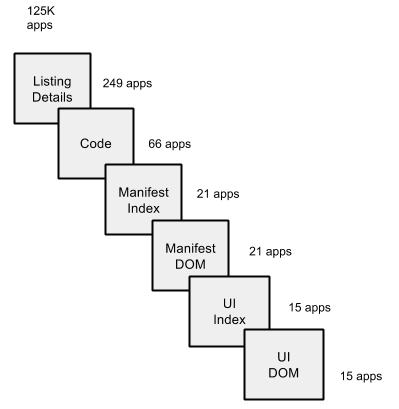
\includegraphics[scale=0.5]{figures/sieveable-deep-search/queryExecution.png}
	\caption{The execution sequence for a query that includes multiple level search conditions.}
	\label{fig:fig_query_execution}
\end{figure}
The query executor creates a plan for executing the received query parts.
The plan is an order of steps to query each index and data store (listing, UI, manifest, and code).
Query parts are executed by collection finder plug-ins (e.g., find by UI Index, find by UI DOM, find by code, etc.).
Collection finders return a set of app ids that matched the given query.
Sieveable computes the intersection of app ids to avoid scanning entire collections.
This also ensures that the final query results only contain ids for apps matched by all query conditions.

Figure~\ref{fig:fig_query_execution} shows the execution sequence of the query in Listing~\ref{lst:query_example} and the number of apps scanned by each collection.
The entire dataset contains over 400,000 apps.
The listing details query part is executed by the \textit{findByListing} module, which returns 249 apps developed by Google and filtered by the latest version of each app.
Next, the \textit{findByCode} module executes the code query part only on those 249 apps and returns 66 apps.
The \textit{findByManifestIndex} module searches the Manifest index for the Manifest query part only on those 66 apps and returns 21 apps.
The Manifest query part is sent to the \textit{findByManifestDOM} module to match the DOM tree for those 21 apps. Since the query part contains no hierarchical structure, the DOM matcher returns the 21 apps found by the index.
Next the UI query part is sent to the UI index to search for apps with LinearLayout and child Button.
The \textit{findByUIIndex} searches the UI index for those 21 apps  and finds that 15 of them have that UI structure.
The UI query part is sent to the \textit{findByUIDOM} module to match the DOM tree for those 15 apps which returns the final query results (15 apps).
Finally, Sieveable returns any field defined in the return clause for the matched app ids.
The return clause in the submitted query includes only a single app field, so Sieveable will return an array of objects where each object contains key-value pairs for the app id, package name, and version code. Below is part of the final query result:
\begin{minted}[fontsize=\footnotesize]{javascript}
[{ "app": { 
"id": "com.google.android.talk-21224130",
"packageName": "com.google.android.talk",
"version": "21224130"
}
}]
\end{minted}

\section{System Implementation}
\begin{figure*}[!t]
	\centering
	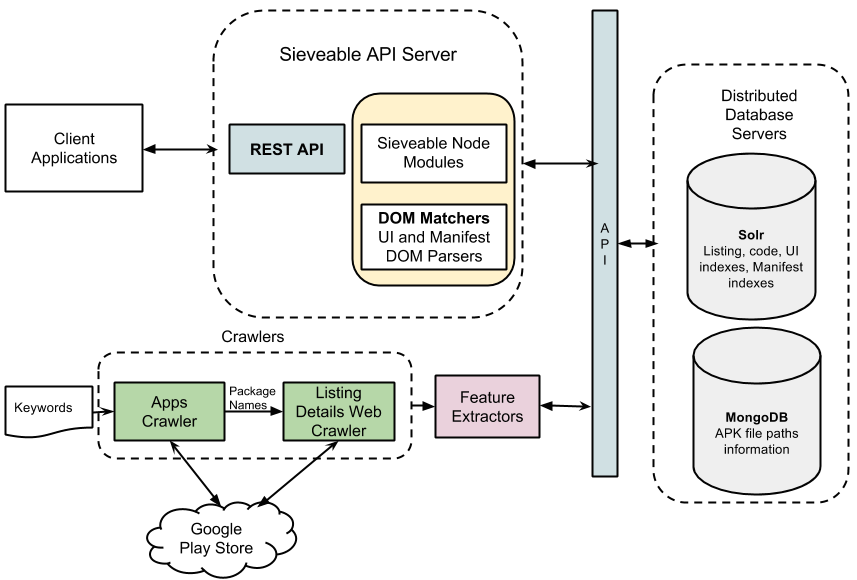
\includegraphics[width=17cm, height=10cm]{figures/sieveable-deep-search/architecture.png}
	\caption{Sieveable system architecture.}
	\label{fig:fig_architecture}
\end{figure*}

In this section, we discuss the technical details of designing and implementing our system. The system consists of six main components: app crawlers, feature extractors, data indexers, data store servers, DOM matchers, and a restful API (see Figure~\ref{fig:fig_architecture}).

\subsection{App Crawlers}
Sieveable features two crawlers that collect our dataset of apps: apps crawler and listing details web page crawler,
The app crawler is responsible for downloading APK files from the Google Play store.
We feed a dictionary of popular Android search keywords into the crawler.
Google has no official API for downloading APK files.
We used an unofficial API\footnote{http://github.com/Akdeniz/google-play-crawler} to collect APK files.
When an APK file is downloaded we run the Android Asset Packaging Tool (aapt) on the file to obtain its package name and version code.
We use a combination of the package name and version code as a unique identifier for each app.
APK files are stored in the file system while their ids and disk paths are stored in a MongoDB collection for fast retrieval.
Once an APK file is downloaded, we run a web crawler to fetch the most recent listing details web page of the app.
We parse the listing details fields and save them in another MongoDB collection.

\subsection{Feature Extractors}
We built a set of command line tools to extract features from the APK files.
First, we use apktool \cite{apktool}, an open-source reverse engineering tool, to decode the apps and obtain their source files.
Second, we run a custom UI parser that parses layout files and resolves any references to external resources (e.g., \texttt{android:text="@string/variable"}) or embedded layouts (using \texttt{<include/>} and \texttt{<merge/>} tags).
The parser produces a single XML file that contains the entire app UI tree, including all files.
This is especially important when performing DOM matching queries since it eliminates the need to load multiple layout files into memory when performing such queries.
Below is a snippet from an XML file generated for the YouTube app.

\begin{minted}{xml}
<App name="com.google.android.youtube" version_code="5021">
    <Directory directory_name="layout">
       <File file_name="activity_feed_item.xml">
          <RelativeLayout>
             <ImageView android:id="@id/channel_avatar"/>
           </RelativeLayout>
           ...
       </File>
    </Directory>
</App>
\end{minted}

Third, we extract all API calls from the smali files, a human readable assembly-like language for the disassembled byte code.
We save the extracted API calls in one text file per app.

\subsection{Data Indexers}
Sieveable indexes the extracted features in Solr collections for fast data access.
A collection is a complete logical index.
We use five Solr logical indexes to index our dataset: listing index, UI tag index, ui structural index, manifest tag index, and code index.

\textbf{Indexing Listing Details:} It contains all listing detail fields. Four fields are indexed as generic text fields (description, title, ``what's new'', and reviews) to support text based search.

\textbf{Indexing UI Data:} The extracted UI files are indexed in two Solr indices: \textit{1) Tag Index:} We extract all tag names and attributes and store them in one index document.
This index holds all tag names and their attributes.
\textit{2) Structural Index:} a suffix tree based index that stores the XML tree in a suffix array format \cite{shasha_2002_atreegrep}.
This index holds values that indicate the parent-child relationship of nodes in the XML tree. (e.g., \path{LinerLayout->Button}).
We parse the single XML UI tree file we extracted for each app and generate two text documents. The first text document contains the tag and attribute names for all UI elements (e.g., \path{EditText(android:layout_width="fill_parent")}).
We add this document to Solr and use it as the tag index.
The second generated document describes the UI tree in a suffix-tree format where each line corresponds to a root-to-leaf path for all XML elements (e.g., \path{RelativeLayout->LinearLayout->ImageButton}).
We add this document to Solr and use it as the structural index.

\textbf{Indexing Manifest Data:} The extracted manifest files are indexed by their tag names and attribute values.
Unlike UI queries, Manifest queries are less structural (e.g., find \path{"android.permission.CAMERA"}).
Therefore, we use the same UI tag index method to add manifest files to the Solr index.

\textbf{Indexing Code Files}, we add the extracted invoked API calls from the smali source code files to Solr.

\subsection{Data Store Servers}
Sieveable uses two main NoSQL database servers:
a) MongoDB \cite{mongodb}: is a document-oriented NoSQL database. It contains a collection for storing information about the downloaded APK files.
b) Apache Solr \cite{solr}: is a document-oriented NoSQL Search Platform.
We use Solr to store distributed collections for listing detail fields, UI tags and attributes, UI structural index, Manifest attributes, and code files.
Due to the large size of our data sets (over 8TB), we found that a single machine is not sufficient to store this large data sets.
Thus, we shard and replicate the collections across a cluster of multiple nodes to improve the system performance and availability.
We use an external Zookeeper \cite{zookeeper} cluster of five nodes to synchronize Solr's configuration and elect leaders.
\subsection{DOM Matchers}

Sieveable UI and Manifest search queries are written in  ``example-based'' syntax.
We implement a custom DOM matchers module to navigate the XML DOM tree and select DOM elements with a particular DOM structure.
The DOM matchers perform a jQuery like DOM manipulation.
While loading DOM files for complex queries is often considered expensive, the use of hierarchical indices reduce the number of false candidates significantly.
However, parsing the DOM for large number of files has an inevitable memory and system resources overhead.
Therefore, Sieveable uses a configurable default limit of 50 results per a given search query and return an inalterable cursor to the client to receive the entire query results.

\subsection{RESTful API}
Client applications can access Sieveable through a RESTful API.
The API provides an HTTP GET request mechanism allowing client applications to submit queries and receive the result as a JSON document.
For an easy query access, Sieveable has both a command line and web client applications that interact with the RESTful API.

\section{Summary}
This chapter presented Sieveable, a multi-view search engine for apps on a large-scale.
It discussed the importance of searching and mining apps across multiple views.
For the first time, Sieveable can help users execute deep search queries (illustrated in Chapter \ref{ch:findings_chapter}) and apply data driven approaches with a holistic view of apps at large-scale that could yield valuable results.
Sieveable has been deployed into a distributed computing infrastructure.
For more information on using Sieveable including source code access, please visit:
\url{http://github.com/sikuli/sieveable}.
